% ***************************************************************************************************
%
%	Szablon pracy magisterskiej dla Politechniki Wrocławskiej w wersji dwustronnej.tojakrissmystagogus
%	Autor:	Tomasz Strzałka
% Koretkta i dostosowanie do wymogów WIT 3.12.2021: dr inż. Anna Lauks-Dutka
%
% ***************************************************************************************************

% Styl dwustronny z domyślną wielkością czcionki 10pt oraz oddzieloną stroną tytułową (titlepage).
% Domyślnie rodziały rozpoczynają się na stronie prawej (openright).
\documentclass[10pt]{book}
\usepackage{times}


% ***************************************************************************************************
% Ustawienia języka
% ***************************************************************************************************

% Podstawowe ustawienia języka, według którego formatowany będzie dokument
\usepackage[polish]{babel}

% Pakiet babel dla polskiego języka powoduje konflikt z pakietem amssymb.
% Polecenie '\lll' definiują oba pakiety - porządana jest druga definicja.
\let\lll\undefined

% W przypadku wielojęzykowości ustawia główny język dokumentu
\selectlanguage{polish}

% Kodowanie dokumentu
\usepackage[utf8]{inputenc}

% Dowolny rozmiar czcionek, kodowanie znaków
\usepackage{lmodern}

% Polskie wcięcia akapitów
\usepackage{indentfirst}

% Polskie łamanie wyrazów
\usepackage[plmath]{polski}

% Przecinek w wyrażeniach matematycznych zamiast kropki
\usepackage{icomma}

% Polskie formatowanie typograficzne
\frenchspacing

% Zapewnia liczne usprawnienia wyświetlania i organizacji matematycznych formuł. 
\usepackage{amsmath}

% Wprowadza rozszerzony zestaw symboli m.in. \leadsto
\usepackage{amssymb}

% Dodatkowa, ,,kręcona'' czcionka matematyczna
\usepackage{mathrsfs}

% Dodatkowe wsparcie dla środowiska mathbb, które nie wspiera domyślnie cyfr (\mathbb{})
\usepackage{bbold}

% Fixes/improves amsmath
\usepackage{mathtools}


% ***************************************************************************************************
% Kolory  
% ***************************************************************************************************

% Umożliwia kolorowanie poszczególnych komórek tabeli
\usepackage[table]{xcolor}% http://ctan.org/pkg/

% Umożliwia łatwą zmianę koloru linii w tabeli
\usepackage{tabu}

% Umożliwia rozszerzoną kontrolę nad kolorami.
\usepackage{xcolor}

% Definicje kolorów
\definecolor{lgray}{HTML}{9F9F9F}
\definecolor{dgray}{HTML}{5F5F5F}
% lgray				-	nazwa nowo zdefiniowanego koloru
% HTML				-	model kolorów
% CCCCCC			-	wartość koloru zgodna z modelem

% ***************************************************************************************************
% Algorytmy 
% ***************************************************************************************************

% Udostępnia środowisko do konstruowania pseudokodów
\usepackage[ruled,vlined,linesnumbered,longend,algochapter]{algorithm2e}
% ruled	- poziome kreski na początku i końcu algorytmu, podpis na górze oddzielony również kreską poziomą
% vlined - pionowe kreski łączące początek polecenia z jego końcem
% linesnumbered	- numerowanie kolejnych wierszy algorytmu
% longend - długie końcówki np. ifend, forend itd.
% algochapter - numeracja z rozdziałami

% Zamiana nazwy środowiska z domyślnej "Algorithm X" na "Pseudokod X"
\newenvironment{pseudokod}[1][htb]{
	\renewcommand{\algorithmcfname}{Pseudokod}
	\begin{algorithm}[#1]%
	}{
\end{algorithm}
}

% Zmiana rozmiaru komentarzy
\newcommand\algcomment[1]{
	\footnotesize{#1}
}

% Ustawienie zadanego stylu dla komentarzy
\SetCommentSty{algcomment}

% Wyśrodkowana tylda
\usepackage{textcomp}%
\newcommand{\textapprox}{\raisebox{0.5ex}{\texttildelow}}

% Listowanie kodów źródłowych
\usepackage{listings} 
\renewcommand{\lstlistingname}{Kod źródłowy} % Polska nazwa listingu

% Definicje pecjalnych znaków, które nie są obsługiwane w środowisku listing
\lstset{literate=
	{ż}{{\.{z}}}1	{ź}{{\'{z}}}1
	{ć}{{\'{c}}}1	{ń}{{\'{n}}}1
	{ą}{{\c a}}1	{ś}{{\'{s}}}1
	{ł}{{\l}}1		{ę}{{\c{e}}}1
	{ó}{{\'{o}}}1	{á}{{\'a}}1
	{é}{{\'e}}1		{í}{{\'i}}1
	{ó}{{\'o}}1		{ú}{{\'u}}1
	{ù}{{\`u}}1		{Á}{{\'A}}1
	{É}{{\'E}}1		{Í}{{\'I}}1
	{Ó}{{\'O}}1		{Ú}{{\'U}}1
	{à}{{\`a}}1		{è}{{\'e}}1
	{ì}{{\`i}}1		{ò}{{\`o}}1
	{ò}{{\`o}}1		{À}{{\`A}}1
	{È}{{\'E}}1		{Ì}{{\`I}}1
	{Ò}{{\`O}}1		{Ò}{{\`O}}1
	{ä}{{\"a}}1		{ë}{{\"e}}1
	{ï}{{\"i}}1		{ö}{{\"o}}1
	{ü}{{\"u}}1		{Ä}{{\"A}}1
	{Ë}{{\"E}}1		{Ï}{{\"I}}1
	{Ö}{{\"O}}1		{Ü}{{\"U}}1
	{â}{{\^a}}1		{ê}{{\^e}}1
	{î}{{\^i}}1		{ô}{{\^o}}1
	{û}{{\^u}}1		{Â}{{\^A}}1
	{Ê}{{\^E}}1		{Î}{{\^I}}1
	{Ô}{{\^O}}1		{Û}{{\^U}}1
	{œ}{{\oe}}1		{Œ}{{\OE}}1
	{æ}{{\ae}}1		{Æ}{{\AE}}1
	{ß}{{\ss}}1		{ç}{{\c c}}1
	{Ç}{{\c C}}1	{ø}{{\o}}1
	{å}{{\r a}}1	{Å}{{\r A}}1
	{€}{{\EUR}}1	{£}{{\pounds}}1
}

% ***************************************************************************************************
% Marginesy 
% ***************************************************************************************************

% Ustawienia rozmiarów stron i ich marginesów
%korekta ALD - dodatkowe 0.5cm na oprawę z lewej
%\usepackage[headheight=18pt, top=25mm, bottom=25mm, left=25mm, right=25mm]{geometry}
\usepackage[headheight=18pt, top=25mm, bottom=25mm, left=30mm, right=25mm]{geometry}
% headheight		-	wysokość tytułów
% top				-	margines górny
% bottom			-	margines dolny
% left				-	margines lewy
% right				-	margines prawy

% Usunięcie górnego marginesu dla środowisk
\makeatletter
\setlength\@fptop{0\p@}	
\makeatother

% ***************************************************************************************************
% Styl 
% ***************************************************************************************************

% Definiuje środowisko 'titlingpage', które zapewnia pełną kontrolę nad układem strony tytułowej.
\usepackage{titling}


% Umożliwia modyfikowanie stylu spisu treści
\usepackage{tocloft}	

\tocloftpagestyle{tableOfContentStyle}

% Definiowanie własnych stylów nagłówków i/lub stopek
\usepackage{fancyhdr}

% Domyślny styl dla pracy 
\fancypagestyle{custom}{
	\fancyhf{}									% wyczyść stopki i nagłówki
	\fancyhead[RO]{								% Prawy, nieparzysty nagłówek
%korekta ALD: 
%\hrulefill \hspace{16pt} \large Rozdział \thechapter
		\hrulefill \hspace{16pt} \large \ifnum \thechapter>0 {Rozdział \thechapter} \else{Wstęp}\fi
		\put(-472.1, 12.1){%
			\makebox(0,0)[l]{%
                
\includegraphics[width=0.05\textwidth]{img/pwr-logo}
			}
		}
		\put(-443,5.5){%
			\makebox(0,0)[l]{%
				\small Politechnika Wrocławska
			}
		}
	}
	\fancyhead[LE]{								% Lewy, parzysty nagłówek
%korekta ALD: 
%\large Rozdział \thechapter \hspace{16pt} \hrulefill 
        \large \ifnum \thechapter>0 {Rozdział \thechapter} \else{Wstęp}\fi \hspace{16pt} \hrulefill 
		\put(-22, 12.1){%
			\makebox(0,0)[l]{%
                %korekta ALD
				%
\includegraphics[width=0.05\textwidth]{pwr-logo}
                
\includegraphics[width=0.05\textwidth]{img/wit-logo}			}
		}
		\put(-210,5.5){%
			\makebox(0,0)[l]{%
%				\small Wydział Podstawowych Problemów Techniki
%Korekta ALD
\small Wydział Informatyki i Telekomunikacji
			}
		}
	}
	\fancyfoot[LE,RO]{							% Stopki
		\thepage
	}
	\renewcommand{\headrulewidth}{0pt}			% Grubość linii w nagłówku
	\renewcommand{\footrulewidth}{0.2pt}		% Grubość linii w stopce
}


% Domyślny styl dla bibliografii
\fancypagestyle{bibliographyStyle}{
	\fancyhf{}									% wyczyść stopki i nagłówki
	\fancyhead[RO]{								% Prawy, nieparzysty nagłówek
		\hrulefill \hspace{16pt} \large Dodatek \thechapter
		\put(-472.1, 12.1){%
			\makebox(0,0)[l]{%
	
\includegraphics[width=0.05\textwidth]{img/pwr-logo}
			}
		}
		\put(-443,5.5){%
			\makebox(0,0)[l]{%
				\small Politechnika Wrocławska
			}
		}
	}
	\fancyhead[LE]{								% Lewy, parzysty nagłówek
		\large Bibliografia \hspace{16pt} \hrulefill 
		\put(-22, 12.1){%
			\makebox(0,0)[l]{%
			%korekta ALD	\includegraphics[width=0.05\textwidth]{wppt-logo}
			
\includegraphics[width=0.05\textwidth]{img/wit-logo}
			}
		}
		\put(-210,5.5){%
			\makebox(0,0)[l]{%
			%korekta ALD
				%\small Wydział Podstawowych Problemów Techniki
				\small Wydział Informatyki i Telekomunikacji
			}
		}
	}
	\fancyfoot[LE,RO]{							% Stopki
		\thepage
	}
	\renewcommand{\headrulewidth}{0pt}			% Grubość linii w nagłówku
	\renewcommand{\footrulewidth}{0.2pt}		% Grubość linii w stopce
}

% Domyślny styl dla spisu tabel i rysunków
\fancypagestyle{listOfTablesStyle}{
	\fancyhf{}									% wyczyść stopki i nagłówki
	\fancyhead[RO]{								% Prawy, nieparzysty nagłówek
		\hrulefill \hspace{16pt} \large Spis tabel
		\put(-472.1, 12.1){%
			\makebox(0,0)[l]{%
			
\includegraphics[width=0.05\textwidth]{img/pwr-logo}
			}
		}
		\put(-443,5.5){%
			\makebox(0,0)[l]{%
				\small Politechnika Wrocławska
			}
		}
	}
	\fancyhead[LE]{								% Lewy, parzysty nagłówek
		\large Spis tabel \hspace{16pt} \hrulefill 
		\put(-22, 12.1){%
			\makebox(0,0)[l]{%

\includegraphics[width=0.05\textwidth]{img/wit-logo}
			}
		}
		\put(-210,5.5){%
			\makebox(0,0)[l]{%
				\small Wydział Informatyki i Telekomunikacji
			}
		}
	}
	\fancyfoot[LE,RO]{							% Stopki
		\thepage
	}
	\renewcommand{\headrulewidth}{0pt}			% Grubość linii w nagłówku
	\renewcommand{\footrulewidth}{0.2pt}		% Grubość linii w stopce
}

\fancypagestyle{listOfPlotsStyle}{
	\fancyhf{}									% wyczyść stopki i nagłówki
	\fancyhead[RO]{								% Prawy, nieparzysty nagłówek
		\hrulefill \hspace{16pt} \large Spis rysunków
		\put(-472.1, 12.1){%
			\makebox(0,0)[l]{%
			
\includegraphics[width=0.05\textwidth]{img/pwr-logo}
			}
		}
		\put(-443,5.5){%
			\makebox(0,0)[l]{%
				\small Politechnika Wrocławska
			}
		}
	}
	\fancyhead[LE]{								% Lewy, parzysty nagłówek
		\large Spis rysunków \hspace{16pt} \hrulefill 
		\put(-22, 12.1){%
			\makebox(0,0)[l]{%

\includegraphics[width=0.05\textwidth]{img/wit-logo}
			}
		}
		\put(-210,5.5){%
			\makebox(0,0)[l]{%
				\small Wydział Informatyki i Telekomunikacji
			}
		}
	}
	\fancyfoot[LE,RO]{							% Stopki
		\thepage
	}
	\renewcommand{\headrulewidth}{0pt}			% Grubość linii w nagłówku
	\renewcommand{\footrulewidth}{0.2pt}		% Grubość linii w stopce
}

% Domyślny styl dla dodatków
\fancypagestyle{appendixStyle}{
	\fancyhf{}									% wyczyść stopki i nagłówki
	\fancyhead[RO]{								% Prawy, nieparzysty nagłówek
		\hrulefill \hspace{16pt} \large Załącznik \thechapter
		\put(-472.1, 12.1){%
			\makebox(0,0)[l]{%

\includegraphics[width=0.05\textwidth]{img/pwr-logo}
			}
		}
		\put(-443,5.5){%
			\makebox(0,0)[l]{%
				\small Politechnika Wrocławska
			}
		}
	}
	\fancyhead[LE]{								% Lewy, parzysty nagłówek
		\large Załącznik \thechapter \hspace{16pt} \hrulefill 
		\put(-22, 12.1){%
			\makebox(0,0)[l]{%
%korekta ALD:				\includegraphics[width=0.05\textwidth]{wppt-logo}

\includegraphics[width=0.05\textwidth]{img/wit-logo}
			}
		}
		\put(-210,5.5){%
			\makebox(0,0)[l]{%
			%korekta ALD
				%\small Wydział Podstawowych Problemów Techniki
				\small Wydział Informatyki i Telekomunikacji
			}
		}
	}
	\fancyfoot[LE,RO]{							% Stopki
		\thepage
	}
	\renewcommand{\headrulewidth}{0pt}			% Grubość linii w nagłówku
	\renewcommand{\footrulewidth}{0.2pt}		% Grubość linii w stopce
}

% Osobny styl dla stron zaczynających rozdział/spis treści itd. (domyślnie formatowane jako "plain")
\fancypagestyle{chapterBeginStyle}{
	\fancyhf{}%
	\fancyfoot[LE,RO]{
		\thepage
	}
	\renewcommand{\headrulewidth}{0pt}
	\renewcommand{\footrulewidth}{0.2pt}
}

% Styl dla pozostałych stron spisu treści
\fancypagestyle{tableOfContentStyle}{
	\fancyhf{}%
	\fancyfoot[LE,RO]{
		\thepage
	}
	\renewcommand{\headrulewidth}{0pt}
	\renewcommand{\footrulewidth}{0.2pt}
}
% Formatowanie tytułów rozdziałów i/lub sekcji
\usepackage{titlesec}

% Formatowanie tytułów rozdziałów
\titleformat{\chapter}[hang]					% kształt
{
	\vspace{-10ex}
	%\Huge
	\large
	\bfseries
}												% formatowanie tekstu modyfikowanego elementu
{}												% etykieta występująca przed tekstem modyfikowanego elementu, niewidoczna w spisie treści
{
	10pt
}												% odstęp formatowanego tytułu od lewego marginesu/etykiety
{
    \large
	\bfseries
}												% formatowanie elementów przed modyfikowanym tytułem
[
\vspace{2ex}
%\rule{\textwidth}{0.4pt}
%\vspace{-4ex}
]												% dodatkowe formatowanie stosowane poniżej modyfikowanego tytułu


% Formatowanie tytułów sekcji
\titleformat{\section}[hang]					% kształt
{
	\vspace{2ex}
%	\titlerule\vspace{1ex}
	\large\bfseries
}												% formatowanie tekstu modyfikowanego elementu
{
	\thesection									% etykieta występująca przed tekstem modyfikowanego elementu, niewidoczna w spisie treści
}
{
	0pt
}												% odstęp formatowanego tytułu od lewego marginesu/etykiety
{
	\large
	\bfseries
}												% formatowanie elementów przed modyfikowanym tytułem


%ALD- ustawienia wielkości fontów dla rozdziałów i sekcji
\usepackage{sectsty}
%\chapterfont{\fontsize{14}{17.6}\selectfont}
\sectionfont{\fontsize{13}{16.8}\selectfont}
\subsectionfont{\fontsize{12}{15.6}\selectfont}

% ***************************************************************************************************
% Linki
% ***************************************************************************************************

% Umożliwia wstawianie hiperłączy do dokumentu
\usepackage{hyperref}							% Aktywuje linki

\hypersetup{
	colorlinks	=	true,					% Koloruje tekst zamiast tworzyć ramki.
	linkcolor		=	blue,					% Kolory: referencji,
        citecolor		=	blue,					% cytowań,
	urlcolor		=	blue					% hiperlinków.
}

% Do stworzenia hiperłączy zostanie użyta ta sama (same) czcionka co dla reszty dokumentu
\urlstyle{same}




% ***************************************************************************************************
% Linki
% ***************************************************************************************************

% Umożliwia zdefiniowanie własnego stylu wyliczeniowego
\usepackage{enumitem}

% Nowa lista numerowana z trzema poziomami
\newlist{myitemize}{itemize}{3}

% Definicja wyglądu znacznika pierwszego poziomu
\setlist[myitemize,1]{
	label		=	\textbullet,
	leftmargin	=	4mm}

% Definicja wyglądu znacznika drugiego poziomu
\setlist[myitemize,2]{
	label		=	$\diamond$,
	leftmargin	=	8mm}

% Definicja wyglądu znacznika trzeciego poziomu
\setlist[myitemize,3]{
	label		=	$\diamond$,
	leftmargin	=	12mm
}

% ***************************************************************************************************
% Inne pakiety
% ***************************************************************************************************

% Dołączanie rysunków
\usepackage{graphicx}

% Figury i przypisy
\usepackage{caption}
\usepackage{subcaption}

% Umożliwia tworzenie przypisów wewnątrz środowisk
\usepackage{footnote}

% Umożliwia tworzenie struktur katalogów
\usepackage{dirtree}

% Rozciąganie komórek tabeli na wiele wierszy
\usepackage{multirow}

% Precyzyjne obliczenia szerokości/wysokości dowolnego fragmentu wygenerowanego przez LaTeX
\usepackage{calc}

% ***************************************************************************************************
% Matematyczne skróty
% ***************************************************************************************************

% Skrócony symbol liczb rzeczywistych
\newcommand{\RR}{\mathbb{R}}

% Skrócony symbol liczb naturalnych
\newcommand{\NN}{\mathbb{N}}

% Skrócony symbol liczb wymiernych
\newcommand{\QQ}{\mathbb{Q}}

% Skrócony symbol liczb całkowitych
\newcommand{\ZZ}{\mathbb{Z}}

% Skrócony symbol logicznej implikacji
\newcommand{\IMP}{\rightarrow}

% Skrócony symbol  logicznej równoważności
\newcommand{\IFF}{\leftrightarrow}

% ***************************************************************************************************
% Środowiska
% ***************************************************************************************************

% Środowisko do twierdzeń
\newtheorem{theorem}{Twierdzenie}[chapter]

% Środowisko do lematów
\newtheorem{lemma}{Lemat}[chapter]

% Środowisko do przykładów
\newtheorem{example}{Przykład}[chapter]

% Środowisko do wniosków
\newtheorem{corollary}{Wniosek}[chapter]

% Środowisko do definicji
\newtheorem{definition}{Definicja}[chapter]

% Środowisko do dowodów
\newenvironment{proof}{
	\par\noindent \textbf{Dowód.}
}{
\begin{flushright}
	\vspace*{-6mm}\mbox{$\blacklozenge$}
\end{flushright}
}

%ALD - nowe środowisko do streszczenia i abstractu
\newenvironment{streszczenie}{
	\par\noindent {\large \textbf{Streszczenie}\\[14pt]\indent}
}{}
\newenvironment{abstract}{
	\par\noindent {\large \textbf{Abstract}\\[14pt]\indent}
}{}

% Środowisko do uwag
\newenvironment{remark}{
	\bigskip \par\noindent \small \textbf{Uwaga.}
}{
\begin{small}
	\vspace*{4mm}
\end{small}
}

% ***************************************************************************************************
% Słownik
% ***************************************************************************************************

% Prawidłowe dzielenie wyrazów
\hyphenation{wszy-stkich ko-lu-mnę każ-da od-leg-łość
	dzie-dzi-ny dzie-dzi-na rów-nych rów-ny
	pole-ga zmie-nna pa-ra-met-rów wzo-rem po-cho-dzi
	o-trzy-ma wte-dy wa-run-ko-wych lo-gicz-nie
	skreś-la-na skreś-la-ną cał-ko-wi-tych wzo-rów po-rzą-dek po-rząd-kiem
	przy-kład pod-zbio-rów po-mię-dzy re-pre-zen-to-wa-ne
	rów-no-waż-ne bi-blio-te-kach wy-pro-wa-dza ma-te-ria-łów
	prze-ka-za-nym skoń-czo-nym moż-esz na-tu-ral-na cią-gu tab-li-cy
	prze-ka-za-nej od-po-wied-nio}

% ***************************************************************************************************
% Dokument
% ***************************************************************************************************

\frontmatter

\begin{document}

    \pagestyle{empty}
	\begin{titlingpage}
		\vspace*{\fill}
		\begin{center}
			\begin{picture}(430,500)
				\put(60,590){\makebox(0,0)[l]{\huge \textbf{Politechnika Wrocławska}}}
				\put(40,565){\makebox(0,0)[l]{\Large \textbf{Wydział Informatyki i Telekomunikacji}}}
                \put(0,550){\line(1,0){430}}
                \put(0,510){\makebox(0,0)[l]{\large Kierunek: \textbf{INF-PPT}}}
                %\textbf{3 literowy kod kierunku}}}
                \put(0,490){\makebox(0,0)[l]{\large Specjalność: \textbf{-}}}                
                %\textbf{3 literowy kod specjalności}}}                
				\put(0,370){\begin{minipage}{0.9\textwidth}
				\centering
				\Huge \textsc{Praca Dyplomowa\\ Inżynierska}
                \end{minipage}
				}
% Tytuł pracy
				\put(0,230){\begin{minipage}{0.9\textwidth}
				\centering
				\LARGE \textbf{Serwis do przeprowadzania rozgrywek Rummikub}
                \end{minipage}
				}
% Autor pracy
				\put(0,170){\begin{minipage}{0.9\textwidth}
				\centering
				\Large {
				Adam Bednarz
				}
				\end{minipage}
				}
% dane promotora
				\put(0,90){\begin{minipage}{0.9\textwidth}
				\centering
				\large{
				Opiekun pracy\\
				\textbf{dr inż. Jakub Lemiesz}
				}
				\end{minipage}
				}
				\put(0,-30){
				\begin{minipage}{0.9\textwidth}
				% \normalsize{
				% Słowa kluczowe: 3 do 6 słów kluczowych 
				% }
				\end{minipage}
				}
                \put(0,-80){\line(1,0){430}}
				\put(155,-100){\makebox(0,0)[bl]{\large \textsc{Wrocław 2022}}}
			\end{picture}
		\end{center}	
		\vspace*{\fill}
	\end{titlingpage}
	
    \cleardoublepage
	\begin{streszczenie}
Tutaj tekst streszczenia po polsku. 
\end{streszczenie}

	\vspace*{1cm}	
    \begin{abstract}
The aim of the thesis was to create a service that allows playing Rummikub between players or between a player and a bot. An Android phone app has been created, as well as a browser-based website. Moreover, an algorithm for the bot was described along with complexity analysis. Flutter and Firebase technologies were used during the implementation of the service. Flutter is a technology that allows projects to be created simultaneously for different platforms. Firebase offers server services for the project.
\end{abstract}


    \cleardoublepage
	\pagenumbering{Roman}
	\pagestyle{tableOfContentStyle}
	\tableofcontents

	% spis rysunków (opcjonalnie)    
	% \clearpage
	% \pagestyle{listOfPlotsStyle}
    %    \listoffigures
    %    \addcontentsline{toc}{chapter}{Spis rysunków}
        
        % spis tabel (opcjonalnie)
    %    \clearpage
    %    \renewcommand{\listtablename}{Spis tabel}    
    %    \pagestyle{listOfTablesStyle}
	% \listoftables
	% \addcontentsline{toc}{chapter}{Spis tabel}




    \cleardoublepage
    
		
	% ***************************************************************************************************
	% Wstęp
	% ***************************************************************************************************
	
	\pagestyle{custom}
	\mainmatter
	
	% ***************************************************************************************************
	% Rodziały
	% ***************************************************************************************************

	%Korekta ALD - nienumerowany wstęp
%\chapter{Wstęp}
\addcontentsline{toc}{chapter}{Wstęp}
\chapter*{Wstęp}

\thispagestyle{chapterBeginStyle}

Celem pracy jest zaprojektowanie i implementacja serwisu informatycznego, który umożliwia przeprowadzanie gier Rummikub.
\\

Założenia funkcjonalne serwisu:
	\begin{itemize}
		\item autoryzacja użytkowników,
		\item zarządzanie instancjami gier,
		\item korzystanie z serwisu za pomocą strony internetowej lub aplikacji na telefon,
		\item rozgrywka z botem. \\
	\end{itemize} 

Obecnie istnieją już takie rozwiązania, które dostarczają nam podobne funkcjonalności. Jednakże motywacją tej pracy jest bliższe zapoznanie się z procesem tworzenia takiego serwisu, jak również analiza złożoności gry Rummikub. Czynnikiem wyróżniającym się stworzonego serwisu jest umożliwienie graczom uczestniczenie w danej rozgrywce niezależnie od tego czy korzystają z aplikacji na telefon (iOS, Android), czy też ze strony internetowej w przeglądarce. \\

Praca składa się z czterech rozdziałów. W rozdziale pierwszym omówiono grę Rummikub, jej zasady oraz przebieg rozgrywki. W rozdziale drugim zobrazowano szczegółowy projekt serwisu. Do graficzego przedstawienia wykorzystano notacje UML. W rozdziale trzecim przedstawiono implementację serwisu. Opisane zostały użyte technologie oraz języki programowania, które zostały użyte w projekcie informatycznym. Przedstawiono dokumentację techniczną modułów systemu oraz schemat bazy danych.
	\cleardoublepage

	\chapter{Opis gry Rummikub}
\thispagestyle{chapterBeginStyle}
\label{rozdzial1}

\section{Gra}

Została stworzona przez Ephraima Hertzano i po raz pierwszy wydano ją w 1950 roku. W rozgrywce może uczestniczyć od dwóch do czterech graczy. Gra składa się z kości, które są numerowane od 1 do 13. Występują one w czterech kolorach (pomarańczowy, czerwony, niebieski, czarny). Każda kość o danym kolorze i liczbie występuje dwa razy. Ponadto występują dwie specjalne kości jako jokery. Łącznie gra zawiera 106 kości. \\

Gra polega na wykładaniu grup, bądź serii. Grupa to trzy lub cztery kości o różnych barwach, ale z tą samą liczbą, natomiast seria to co najmniej trzy kolejne kości o tym samym kolorze. \\

W przypadku braku odpowiednich kości do gry można posłużyć się dwoma zestawami kart po 52 karty i 2 jokery. Gdzie 1, 11, 12, 13 można zastąpić odpowednio asem, waletem, damą i królem.

\section{Rozgrywka}

Zbiór wszystkich wymieszanych kości nazywany jest bankiem. Z niego na początku gry każdy gracz otrzymuje 14 kości. W przypadku pierwszego ruchu należy wyłożyć własne kości o sumie numerów tych kości co najmniej 30, bez możliwości modyfikowania kości leżących na planszy. \\

Po wyłożeniu pierwszego ruchu gracz może modyfikować inne wyłożone wcześniej układy. Dozwolone jest przebudowywanie układów kości (rozbijanie lub rozbudowywanie). Jednak w każdym ruchu należy wyłożyć przynajmniej jedną własną kość. \\

Na każdy ruch przypada ustalony wcześniej limit czasowy. Po jego upływie w przypadku braku wyłożenia kości przez gracza, lub gdy stan planszy nie spełnia zasad gry, gracz pobiera z banku jedną kość i cofa wprowadzone zmiany układów kości. \\

Joker w grze Rummikub symbolizuje dowolną kość. Można nim zastąpić brakujący element do utworzenia układu kości. Joker ma taką samą wartość jak kość, którą zastępuje. Można zabrać wyłożonego jokera zastępując go odpowiednią kością i wykorzystać go w innym miejscu na planszy. \\

Gra kończy się w momencie, gdy któryś z graczy wyłoży wszystkie swoje kości lub gdy zabraknie kości w banku. W przypadku drugim wygrywa ten gracz, który ma najmniejszą sumę liczb znajdujących się na kościach.



	\cleardoublepage

	\chapter{Projekt serwisu}
\thispagestyle{chapterBeginStyle}

W tym rozdziale przedstawiono szczegółowy projekt systemu w notacji UML uwzględniający wymagania funkcjonalne opisane we wstępie. Do opisu relacji pomiędzy składowymi systemu wykorzystano diagramy UML.

\section{Struktura}

W serwisie wykorzystano architekturę klient-serwer. Istnieje jeden serwer, do którego może podłączać się wiele klientów i odpowiada on za komunikację i zarządzanie danymi.
W komponencie klienta wykorzystano architekturę trójwarstwową. Architektura ta dzieli komponent na trzy osobne części:
\begin{itemize}
	\item warstwa prezentacji,
	\item warstwa biznesowa,
	\item warstwa danych.
\end{itemize}
Warstwa prezentacji jest to interfejs graficzny użytkownika. Jest odpowiedzialna za interakcję z użytkownikiem (wyświetlanie i wprowadzanie danych). \\ \\
Warstwa biznesowa odpowiada za przetwarzanie komunikatów od użytkownika lub ze strony serwera. Tutaj zawarta jest wszelka logika aplikacji. Przetworzone dane są przekazywane do warstwy prezentacji i/lub warstwy danych. Warstwa ta jest łącznikiem pomiędzy warstwą prezentacji, a warstwą danych. \\ \\
Warstwa danych jest dostępem do danych. Obsługuje połączenie aplikacji z zewnętrznym obiektem dostarczającym dane (baza danych, serwer).

\section{Przypadki użycia i scenariusze}



\section{Diagramy aktywności}


\section{Diagramy stanów}





	\cleardoublepage
	
	\chapter{Opis technologii}
\thispagestyle{chapterBeginStyle}

W rozdziale tym wskazano jakie podejście technologiczne zostało użyte wraz z omówieniem i zaargumentowaniem powodu takiego wyboru. Przedstawiono również jakie konkretne aspekty tych technologii zostały wykorzystane w projekcie.

\section{Flutter}

Do implementacji serwisu po stronie klienta użyto technologii Flutter. Jest to zestaw narzędzi pozwalający tworzyć natywne, wieloplatformowe aplikacje mobilne, komputerowe oraz internetowe. Flutter stworzony jest przez firmę Google, a jego pierwsza stabilna wersja ukazała się pod koniec 2019 roku. Mimo stosunkowo młodej technologii Google przyczynia się do jej dynamicznego rozwoju i zdobywania popularności wśród programistów. 

\subsection{Dart}

Aplikacje we Flutterze pisze się w języku Dart. Jest to zorientowany obiektowo, statycznie typowany, wysokopoziomowy język programowania. Składnia języka Dart wzorowana była na takich językach programowania jak Java czy C\#, by ułatwić programistom naukę języka. Ze względu na to, że jest to dosyć nowy język, warto uwzględnić tutaj parę charakterystycznych cech, co może być przydatne w zapoznawaniu się z kodem źródłowym tego serwisu. \\

Funkcja \emph{main()} jest punktem wejścia do programu napisanego za pomocą Dart, zatem język ten nie wymaga klasy (w przeciwieństwie do Java). Wszystko, co można umieścić we zmiennej, jest obiektem. Oprócz ogólnych typów danych, istnieje typ \emph{dynamic}. Zmiennna tego typu może zawierać dowolny typ. Wszystkie typy są domyślnie \emph{non-nullable}, więc muszą zawierać jakąś wartość. Jeśli chcemy zadeklarować zmienną z pustą wartością, po nazwie typu umieszczamy \emph{"?"} np. \emph{int?}. Dart używa wnioskowania o typie, więc zaleca się deklarowanie zmiennych z użyciem słowa kluczowego \emph{var} lub \emph{final} czy \emph{const}. W języku tym nie występują słowa kluczowe \emph{public}, \emph{protected}, \emph{private}. Domyślnie wszystkie zmienne są publiczne, jeśli jednak nazwa zmiennej będzie zaczynać się od \emph{,,\_''}, to będzie to zmienna prywatna. Podczas tworzenia obiektów używanie słowa \emph{new} jest opcjonalne. W konstruktorze można odwołać się do zmiennych instancji, aby automatycznie przypisać im wartości np. \emph{MojaKlasa(this.zmienna1, this.zmienna2);} Dodatkowo każda klasa ma domyślne metody \emph{set} do modifikowania danej zmiennej oraz \emph{get} do jej zwracania. W przypadku zmiennych prywatnych \emph{getter} nie występuje, a w przypadku stałych \emph{setter} nie występuje. \\

W implementacji serwisu często korzystano z programowania asynchronicznego. W języku Dart programowanie to charakteryzuje się klasami \emph{Future} oraz \emph{Stream}. Obie klasą umożliwiają wykonywanie kodu asynchronicznie. W przypadku \emph{Future} wykonuje się jedno zapytanie i zwracana zostaje odpowiedź. Natomiast w przypadku \emph{Stream} na jedno zapytanie może być zwracane wiele odpowiedzi.

\subsection{Widget}

Każdy element interfejsu użytkownika we Flutterze jest widgetem. Widget może być elementem widocznym np. przyciskiem, ale również niewidocznym, który będzie odpowiadał za definiowanie układu elementów jak np. kolumna. Są dwa typy widgetów: statyczny oraz dynamiczny. W statycznym widgecie wszystkie pola muszą być stałe. W przypadku widgetów dynamicznych za każdym razem, gdy jego stan się zmienia jest przebudowywany. Interfejs buduje się  poprzez zagnieżdżanie widgetów. Zatem cała strona bądź ekran jest widgetem jako całość, ale ta całość składa się z innych widgetów. \\

Ważnym aspektem w interfejsie użytkownika jest przechodzenie pomiędzy ekranami czy stronami. W Flutterze za ten mechanizm odpowiada \emph{Navigator}, który należy do widgetów niewidocznych oraz obiekt \emph{Route}. \emph{Navigator} zarządza obiektami \emph{Route} na stosie. Natomiast \emph{Route} jest obiektem reprezentującym daną stronę czy ekran. Przesyłając do \emph{Navigatora} obiekt \emph{Route}, widget znajdujący się w tym obiekcie będzie umieszczany na stosie, więc tylko on będzie widoczny jako interfejs użytkownika. Zatem cofnięcie się w tył w aplikacji, będzie zrzucało dany widget ze stosu i będzie widoczny poprzedni widget.

\subsection{BLoC}

Flutter domyślnie nie oddziela kodu dotyczącego sposobu działania programu od części wizualnej. Chcąc wyodrębnić aspekty wizualne od aspektów logicznych aplikacji, należy użyć wybranego wzorca architektury. Istnieje wiele pakietów pomagających zaimplementować poszczególne wzorce. W tym projekcie zastosowano rekomendowany przez Google pakiet BLoC, który umożliwia implementacje architektury trójwarstwowej z podziałem na warstwę wizualną, logiki i danych, jak również wprowadza system zarządzania stanami w aplikacji. \\

\begin{figure}[h!]
	\begin{center}
		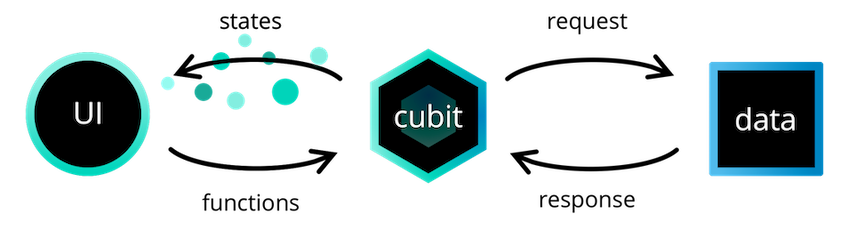
\includegraphics[width=1\textwidth]{img/cubit.png}
	\end{center}
	\caption{{\color{dgray}Model struktury wzorca projektowego BLoC.}} 
	\label{struktura_BLoC}
\end{figure}  

BLoC (Business Logic Component) - wzorzec projektowy pomagający oddzielić elementy wizualne projektu od części logiki działania programu. Dzieli projekt na trzy główne komponenty UI, cubit, data.

Warstwa UI jest odpowiedzialna za część wizualną aplikacji, cubit jest warstwą zawierającą mechanizmy działania aplikacji oraz pomostem pomiędzy interfejsem użytkownika, a zewnętrznymi danymi, natomiast warstwa data komunikuje się z zewnętrznymi instancjami (serwer, baza danych).\\

Cubit komunikuje się z warstwą danych poprzez funkcje asynchroniczne. Natomiast chcąc wpłynąć na zmianę wyglądu aplikacji korzysta z programowania reaktywnego. Mianowicie wysyła poszczególne stany strumieniem, którego dany element interfejsu aplikacji nasłuchuje. Stan jest to klasa reprezentująca dany stan poszczególnego elementu aplikacji. Relacja w drugą stronę polega na wywoływaniu bezpośrednio funkcji (synchronicznej lub asynchronicznej) na instancji cubita.

\section{Firebase}

Rolę serwera i bazy danych pełni platforma Firebase. Technologia ta, zarządzana również przez Google, określana jest jako Backend-as-a-Service. Firebase dostarcza wiele funkcjonalności wspierające tworzenie projektów w tym między innymi uwierzytelnianie użytkowników, bazę danych NoSQL oraz API odpowiedzialne za komunikację. Usługi, które świadczy Firebase są bezpłatne, jeśli nie przekroczą pewnego z góry ustalonego limitu zdefiniowanego dla poszczególnej funkcjonalności. 

\subsection{Firestore}

Firestore jest to baza danych NoSQL w chmurze. Jej strukturą są kolekcje, które zawierają dokumenty, które te z kolei zawierają dane, ale także mogą zawierać kolejne kolekcje. \\
Definiując zapytania do bazy danych zwracane są jedynie dokumenty z poszczególnej kolekcji lub grup kolekcji. Firestore umożliwia tworzenie prostych zapytań SQL, które filtruje wyniki na podstawie wartości danych znajdujących się w dokumencie. \\
Firebase umożliwia po stronie klienta implementacje słuchaczy, którzy będą niezwłocznie informowani, gdy w obserwowanym dokumencie zaszła zmiana. \\
Firestore umożliwia konfigurację dostępu do bazy danych za pomocą definiowania reguł bezpieczeństwa. Dla każdego dokumentu oraz pola można zdefiniować zakres dostępu (czytanie, modyfikacja, usuwanie) dla poszczególnego użytkownika.


\subsection{Funkcje Firebase}

Umożliwiają zaimplementowanie własnego kodu po stronie serwera. Są wywoływane poprzez zapytania HTTPS lub w odpowiedzi na zdarzenia powstałe w bazie danych Firestore. \\
Możliwe jest wywoływanie bezpośrednio z poziomu aplikacji. Do zapytania dołączane są tokeny uwierzytelniania Firebase i tokeny sprawdzania aplikacji.

\subsection{Konsola Firebase}

Jest to strona internetowa, która oferuje dostęp do wszystkich funkcjonalności Firebase. Aby korzystać z platformy Firebase należy założyć tam własny projekt i skonfigurować go z docelową aplikacją. Po wstępnej konfiguracji otrzymuje się panel kontroli nad platformą Firebase dla projektu. Widzi się cały ruch generowany przez klientów w poszczególnych funkcjonalnościach np. liczba zapisów do bazy danych. Za pomocą konsoli można konfigurować i modyfikować każdą usługę. Zapewnia bezpośrednio dostęp do bazy danych, zarządzanie zarejestrowanymi użytkownikami, monitorowanie procesu działania serwisu. 

\subsection{Emulator}

Korzystając z funkcjonalności funkcji Firebase napotyka się na problem długiego czasu oczekiwania na zaktualizowanie kodu źródłowego programisty w chmurze Firebase (czas trwania około minuty). Oczekiwanie dłuższe niż parę sekund sprawia, że czas tworzenia kodu źródłowego po stronie serwera znacząco się wydłuża. Kolejną sprawą jest fakt, że w trakcie, gdy dany projekt jest już dostępny dla użytkowników, nie jest wskazana jego modyfikacja. Zatem trzeba tworzyć kopie projektu, które przeznaczone są modyfikacji, co w przypadku, gdy nad projektem pracuje wielu programistów, staje się jeszcze bardziej nieefektywne. Ostatnim aspektem są koszty. W momencie programowania i testowania funkcjonalności serwera może dochodzić do generowania dużej ilości zapytań, co z kolei sumuje się do liczby zapytań i ewentualnych płatności. \\

Z powodu wyżej wymienionych problemów wraz z rozwojem platformy Firebase w 2019 roku oficjalnie został zaprezentowany Firebase Local Emulators. Emulator ten pozwala uruchomić wszystkie usługi Firebase lokalnie na własnym komputerze. Dzięki czemu szybko można nanieść zmiany w funkcjach Firebase, nie modyfikując właściwego projektu, a wykonywane zapytania nie są zliczane. \\

Każda usługa udostępniana przez platformę Firebase ma swój własny emulator, który jest uruchamiany na osobnym porcie. Zatem można uruchomić jedynie te emulatory tych funkcjonalności, które są wykorzystywane w projekcie. Ponadto fakt uruchomienia lokalnie funkcji Firebase  umożliwia debugowanie kodu.




	\cleardoublepage
	
	\chapter{Implementacja serwisu}
\thispagestyle{chapterBeginStyle}

Rozdział ten zawiera dokumentację techniczną projektu. Zobrazowano sposób w jaki założenia projektowe, zostały zaimplementowane przy użyciu wybranych technologii. Zgodnie ze strukturą serwisu w podrozdziale pierwszym opisano sposób implementacji serwera, a podrozdziale drugim klienta. Przedstawiona ogólna dokumentacja miała na celu bliższe zapoznanie się ze sposobem działania serwisu pod względem informatycznym.

\section{Serwer}

Przy implementacji serwera wykorzystano głównie trzy moduły Firebase takie jak uwierzytelnianie, firestore (baza danych NoSQL) oraz funkcje. Komunikacja pomiędzy serwerem, a klientem opiera się na dwóch sposobach. Klient może bezpośrednio nasłuchiwać zmian zachodzących w bazie danych Firestore, albo wywoływać funkcje Firebase.

\subsection{Baza danych}

W bazie danych czasu rzeczywistego Firestore zostały umieszczone dwie kolekcje - \emph{Users}, \emph{Games}. W kolekcji \emph{Users} są przechowywane dokumenty indeksowane unikatowymi kodami ID użytkownika, które są przydzielane w czasie rejestracji. Każdy dokument zawiera pola \emph{name} i \emph{active}. Pole \emph{name} odnosi się do nazwy użytkownika, a pole \emph{active} jest wartością logiczną wskazującą, czy dany użytkownik jest dostępny w grze (jest zalogowany i obecnie nie znajduje się w rozgrywce z innymi graczami). Opcjonalne pole \emph{invitation} jest mapą zawierającą klucze \emph{gameId} oraz \emph{player}, których wartości wskazują kolejno na kod ID gry i nazwę gracza, który zaprosił danego gracza do swojej gry. W kolekcji \emph{Games} są przechowywane dokumenty indeksowane automatycznie generowanymi unikatowymi kodami ID przy tworzeniu dokumentu i które są przypisane jako kody ID gier. Każdy dokument zawiera trzy pola: \emph{available} (wskazuje ile graczy może jeszcze dołączyć do gry), \emph{currentTurn} (wskazuje jakiego gracza jest teraz kolej), \emph{size} (wskazuje na liczbę graczy w grze). Ponadto dokument danej gry zawiera jeszcze subkolekcje \emph{playersQueue}, \emph{playersRacks}, \emph{pool}, \emph{state}. \\ \\
Subkolekcja \emph{playersQueue} jest to zbiór dokumentów indeksowanych kodami ID graczy, którzy uczestniczą w tej grze. Każdy dokument zawiera pole \emph{name} z nazwą gracza oraz pole \emph{initialMeld}, które wskazuje czy dany gracz wyłożył już rozdanie początkowe. \\
Subkolekcja \emph{playersRack} to zbiór dokumentów z automatycznie generowanymi kodami ID. Dokumenty te przedstawiają kości, które są przydzielone graczowi. Każdy dokument zawiera dwa pola \emph{color} oraz \emph{number}. \\ \\
Subkolekcja \emph{pool} to z kolei zbiór dokumentów z automatycznie generowanymi kodami ID. Zbiór tych dokumentów przedstawia bank w grze, czyli wszystkie kości, które nie znajdują się na planszy ani nie są przydzielone do gracza. Każdy dokument ma pola \emph{color} oraz \emph{number}. \\ \\
Subkolekcja \emph{state} zawiera dokładnie jeden dokument \emph{sets} o najbardziej złożonej strukturze. W dokumencie \emph{sets} znajdują się wszystkie zbiory, które są wyłożone na planszy. Struktura tego dokumentu składa się z mapy, w której klucze to pozycja pierwszej kości z danego zbioru na planszy, a więc moment, w którym rozpoczyna się dany zbiór kości. Wartości tej mapy to tablica kości, gdzie każda kość jest w postaci mapy z kluczami \emph{color} i \emph{number}. Taki sposób przedstawienia stanu planszy wynika głównie z optymizacji kosztów modyfikowania bazy danych. Nie rozbito każdego zbioru kości na osobne dokumenty, ponieważ zwiększa to nam liczbę zliczanych zapisów do bazy danych. Ponadto w tym przypadku nie ma potrzeby korzystania z właściwości oferowanych przez dokumenty takie jak śledzenie zmian w danym dokumencie czy możliwość tworzenia prostych zapytań SQL na zbiorze dokumentów.

\subsection{Uwierzytelnianie}

Tak jak wspomniano wyżej występują dwa sposoby komunikacji klienta z serwerem. W przypadku funkcji Firebase do zapytań HTTPS z aplikacji, automatycznie są dołączane tokeny uwierzytelniania. W przypadku nasłuchiwaniu zmian zachodzących w bazie danych lub operacjach zaczytywania i modyfikowania bazy danych Firestore za proces autoryzacji dostępu są odpowiedzialne reguły bezpieczeństwa Firestore. \\ \\
W tym projekcie reguły bezpieczeństwa Firestore są zdefiniowane następująco:
\begin{itemize}
	\item w kolekcji \emph{users} użytkownik ma dostęp jedynie do dokumentu z własnym ID, na którym może wykonywać operacje czytania i modyfikacji,
	\item w kolekcji \emph{games} użytkownik ma dostęp jedynie do dokumentu gry, w którym on sam jest jednym z graczy. W tym dokumencie będzie miał dostęp do pól zdefiniowanych w dokumencie oraz do subkolekcji \emph{playersQueue} oraz \emph{playersRacks}. Co więcej w \emph{playersRacks} będzie miał dostęp jedynie do dokumentu z własnym polem ID. We wszystkich dostępnych miejscach użytkownik ma prawo jedynie wykonywać operacje czytania.
\end{itemize}

\subsection{Funkcje}

Za pomocą funkcji Firebase został zaimplementowany kod serwera serwisu. Jego głównymi zadaniami jest zarządzanie instancjami gier oraz uniemożliwienie prób oszukiwania w czasie rozgrywki przez graczy za pomocą ingerencji w kod źródłowy aplikacji po stronie klienta. \\ \\
Zbiór zdefiniowanych funkcji został uporządkowany w trzy podzbiory. W pierwszym podzbiorze znajdują się wszystkie możliwe do wywołania przez użytkownika funkcje serwera. Drugim podzbiorem jest klasa \emph{GameUtils}, zawierająca statyczne funkcje odpowiedzialne za zarządzanie instancjami gier. Trzecim podzbiorem jest klasa \emph{GameLogic}, zawierająca statyczne funkcje, które odpowiadają za walidację ruchów użytkowników w grze i implementację logiki rozgrywki gry. \\ \\
Charakterystyka funkcji serwera możliwych do wywołania przez użytkownika:
\begin{itemize}
	\item \emph{createGame} - jako paramtry wejściowe przyjmuje ID gracza i jego nazwę, listę nazw graczy zaproszonych do gry oraz czas przeznaczony na wykonanie ruchu w trakcie gry. \\
	Wywołuje ona metodę \emph{createGame} z klasy \emph{GameUtils}. Następnie wyszukuje poszczególnych graczy i informuje ich o zaproszeniu do gry. \\
	Parametrem zwracanym jest ID nowo utworzonej gry.
	\item \emph{searchGame} - jako parametry wejściowe przyjmuje ustawienia gry: liczbę graczy i czas przeznaczony na ruch gracza oraz ID gracza i jego nazwę. \\ 
	Wywołuje funkcję \emph{findGame} z \emph{GameUtils}. Jeśli gra zostanie znaleziona wywoływana jest funkcja \emph{addToGame}. Następnie jeśli gracz zajął ostatnie wolne miejsce w grze, wywoływana jest funkcja \emph{startGame} z \emph{GameUtils}. Jednak jeśli nie znaleziono gry, wywoływana jest funkcja \emph{createGame} z klasy \emph{GameUtils}.	Aby uchronić się przed wyszukiwaniem i modyfikowaniem bazy danych jednocześnie przez kilka wywołań funkcji \emph{searchGame} przez różnych graczy, proces wyszukania gry i zapisu do niej odbywa się poprzez transakcje. \\
	Parametrem wyjściowym jest ID gry.
	\item \emph{addToExistingGame} - jako parametry wejściowe przyjmuje ID gry oraz ID gracza i jego nazwę. \\
	Funkcja szuka instancji gry, a następnie wywołuje \emph{addToGame} z \emph{GameUtils}. Operacje na bazie danych również odbywają się z pomocą transakcji.
	\item \emph{putTiles} - jako parametry wejściowe przyjmuje ID gracza i gry oraz zbiór zbiorów kości znajdujących się na planszy. \\
	Znajduję instancję gry i subkolekcje graczy uczestniczących w niej, a następnie wywołuje metodę \emph{checkTurn} z \emph{GameLogic}. Potem nadaje prawo ruchu kolejnemu graczowi w kolejce. Dalej wywołuje metodę \emph{addNewTiles} z \emph{GameLogic}. Jeśli metoda ta zwróci, że gracz jest zwycięzcą, wskazuje zwycięzcę. Jeśli zwróci, że gracz nie wykonał żadnego ruchu lub próbował oszukiwać, to doda do jego zbioru kości kolejną kość z banku. W przypadku, gdy była to ostatnia kość z banku, to wywołuje metodę \emph{pointTheWinner} z \emph{GameLogic}.
	\item \emph{leftGame} - jako parametry wejściowe przyjmuje ID gracza i gry. \\
	Usuwa gracza z kolejki graczy w grze. Jeśli akurat ten gracz miał prawo ruchu, daje możliwość ruchu następnemu graczowi. \\
\end{itemize}
Charakterystyka funkcji statycznych serwera z klasy \emph{GameUtils}:
\begin{itemize}
	\item \emph{createGame} - tworzy dokument gry w kolekcji \emph{games}. Dodaje założyciela do subkolekcji \emph{playersQueue} oraz tworzy wszystkie możliwe kości w postaci dokumentów i dodaje je do subkolekcji \emph{pool}. \\
	Zwraca ID gry.
	\item \emph{addToGame} - dodaje gracza do istniejącej już gry. \\
	Zwraca ID gry oraz wartość logiczną dotyczącą występowania wolnych miejsc w grze.
	\item \emph{findGame} -  za pomocą parametrów ustawień gry (liczba graczy, czas na ruch) szuka wolnej instancji gry. \\
	Zwraca instancję gry lub null.
	\item \emph{startGame} -  przydziela graczom po 14 kości losowo wybranych z subkolekcji \emph{pool}. Nadaje prawo do wykonania ruchu pierwszego graczowi w subkolekcji \emph{playersQueue}. \\ 
\end{itemize}
Charakterystyka funkcji statycznych serwera z klasy \emph{GameLogic}:
\begin{itemize}
	\item \emph{checkTurn} - sprawdza, czy dany gracz ma prawo wyłożyć kości.
	\item \emph{addNewTiles} - przeprowadza walidację nowego zbioru kości na planszy. Sprawdza, czy zbiory są poprawnie ułożone, czy występują wszystkie poprzednie kości na planszy, czy nowo położone kości należą do gracza. W przypadku wyłożenia początkowego sprawdza czy gracz wyłożył nowe ułożenia o wartości co najmniej 30 punktów oraz czy poprzednie ułożenie nie zostały zmodyfikowane. Po spełnieniu tych warunków usuwa nowo wyłożone kości z puli gracza i modyfikuje stan planszy. W przypadku wyłożenia początkowego odznacza, że zostało wykonane. \\
	Zwraca informację, czy kości zostały poprawnie dodane lub informację, że gracz zwyciężył w przypadku usunięcia wszystkich kości z jego puli.
	\item \emph{getTileFromPool} - wybiera jedną kość z subkolekcji \emph{pool} i przydziela je danemu graczowi. \\
	Zwraca informację, czy w \emph{pool} znajdują się jeszcze dostępne kości.
	\item \emph{pointTheWinner} -  sumuje wszystkie wartości kości w poszczególnych pulach graczy. Wskazuje zwycięzcę lub zwycięzców w przypadku równości sum.
\end{itemize}

\section{Klient}

Warstwa klienta w serwisie napisana we Flutterze jest dostępna jako aplikacja na telefon albo jako strona internetowa. Z uwagi na wieloplatformowość Fluttera kod źródłowy obu wersji klienta jest wspólny z odpowiednimi konfiguracjami i modyfikacjami na poszczególne platformy.

\subsection{Warstwa prezentacji}

W warstwie prezentacji zdefiniowany jest wygląd aplikacji klienta. Warstwa ta składa się z bezstanowych widgetów, które generują interfejs graficzny. Klasy te odpowiadają za odbieranie
komunikatów ze strony użytkownika jak i przekazują lub odbierają komunikaty ze strony logiki aplikacji. Zdarzenia te mogą mieć wpływ na wygląd danego widgeta. Komunikacja pomiędzy poszczególnymi stronami aplikacji jest również zdefiniowana w tej warstwie. \\

Nawigacja pomiędzy stronami odbywa się poprzez dynamiczną nawigacją z wygenerowanymi trasami. Jest to jeden ze sposobów komunikacji we Flutterze, dzięki któremu za cały proces nawigacji odpowiada klasa \emph{app\_router}, a w poszczególnych widgetach podaje się nazwę ścieżki i obiekty do przekazania pomiędzy stronami. Główną zaletą korzystania z tego sposobu jest eliminacja bezpośrednich zależności pomiędzy widgetami. Ponadto zmniejsza się objętość kodu, a sam kod staje się bardziej przejrzysty. \\

\begin{figure}[h!]
	\begin{center}
		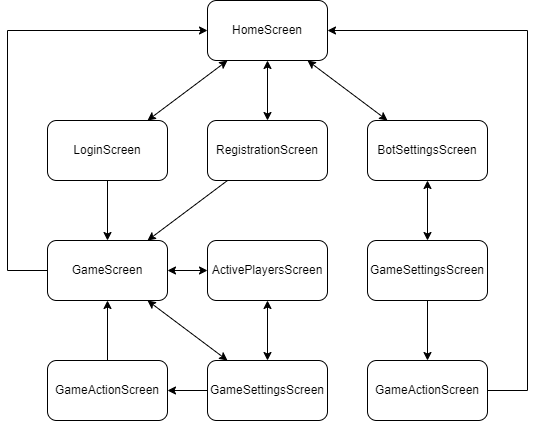
\includegraphics[width=13cm,height=10cm]{img/nawigacja.png}
	\end{center}
	\caption{{\color{dgray}Diagram nawigacji.}} 
	\label{nawigacja}
\end{figure}  

\emph{HomeScreen} jest ekranem startowym aplikacji, od którego zaczyna się każda inna ścieżka. W programie można podążyć dwoma głównymi ścieżkami. Pierwszą ścieżką jest wybranie gry z botem lokalnie na urządzeniu użytkownika bez konieczności połączenia z internetem. Następnie wybraniu ustawień bota i kolejno ustawień gry i przejściu do rozgrywki. Po wyjściu z gry użytkownik wraca do ekranu startowego. Drugą ścieżką jest z kolei zalogowanie się lub utworzenie konta gracza. Następnie użytkownik będzie miał do wyboru sposób rozpoczęcia gry. Jeśli zdecyduje się na utworzenie własnej gry z innymi aktywnymi użytkownikami, przechodzi do strony \emph{ActivePlayersScreen}, a dalej do ustawień gry. Jeśli jednak będzie chciał dołączyć do istniejącej już gry, aplikacja przekierowuje go bezpośrednio do \emph{GameSettingsScreen}. Po przejściu do rozgrywki gracz w każdej chili może opuścić grę. W takim przypadku znajdzie się z powrotem w \emph{GameScreen}. Z którego również może nastąpić wylogowanie się użytkownika i powrót do ekranu startowego. \\ \\ 
Charakterystyka poszczególnych klas w warstwie prezentacji:
\begin{itemize}
	\item \emph{AppRouter} - klasa odpowiadająca za nawigację w aplikacji. Zawiera zdefiniowane ścieżki, które wskazują na poszczególne strony. Jest odpowiedzialna za tworzenie nowego ekranu i dołączanie do niego odpowiednich zależności i przekazywanych parametrów.
	\item \emph{HomeScreen} - klasa zawierająca trzy przyciski kolejno prowadzące do \emph{RegirstrationScreen}, \emph{LoginScreen}, \emph{BotSettingsScreen}. Ekran startowy aplikacji.s
	\item \emph{RegirstrationScreen} - klasa zawierająca formularz z danymi do rejestracji (email, nazwa gracza, hasło, potwierdzenie hasła). Przeprowadza walidację formatu email oraz długości hasła i jego identyczności z potwierdzającym hasłem.
	\item \emph{LoginScreen} - klasa zawierająca formularz z potrzebnymi danymi do zalogowania użytkownika (email, hasło).
	\item \emph{BotSettingsScreen} - klasa zawierająca dwa przyciski, odpowiadające za wybrany poziom bota. Przekierowują one do ekranu \emph{GameSettings} z argumentami \emph{playerId} oraz \emph{serverType}, co w przypadku gry z botem będzie równoznacze z numerem ID gracza \emph{0} oraz typ serwera \emph{basicBot}, \emph{advancedBot}.
	\item \emph{GameScreen} - klasa zawierająca dwa przyciski, które definiują sposób dołączenia do rozgrywki. Prowadzą one do stron \emph{ActivePlayersScreen}, \emph{GameSettingsScreen} i jako parametr przekazują ID gracza. Ponadto, gdy użytkownik chce powrócić do wcześniejszej strony zostanie wyświetlone okno dialogowe, wymuszające potwierdzenie decyzji, gdyż wiążę się ona z wylogowaniem użytkownika i powrotem do ekranu startowego. W przypadku, gdy użytkownik zostanie zaproszony do gry przez innego gracza, również zostanie wyświetlone okno dialogowe, w którym gracz będzie mógł przyjąć lub odrzucić zaproszenie.
	\item \emph{ActivePlayersScreen} - składa się z wyszukiwarki, listy aktywnych użytkowników oraz przycisku. Lista aktywnych użytkowników jest sortowana względem wyrazu wpisanego do wyszukiwarki. Użytkownik wybiera z listy graczy, których chce zaprosić do gry. Po kliknięciu w przycisk przechodzi do \emph{GameSettings} z parametrami \emph{playerId} (ID użytkownika), \emph{selectedPlayers} wybrani gracze, \emph{serverType} (nazwę serwera).
	\item \emph{GameSettingsScreen} - klasa zawierająca dwa pola przeznaczone do konfiguracji liczby uczestników i czasu przeznaczonego na ruch gracza oraz przycisk. Po kliknięciu w przycisk ukazuje się obracające kółeczko i napis z liczbą graczy brakujących do rozpoczęcia rozgrywki. Po pojawieniu się wymaganej liczby graczy nastąpi przekierowanie do \emph{GameActionScreen} z parametrami \emph{gameId}, \emph{playerId}, \emph{serverType}.
	\item \emph{GameActionScreen} - klasa obrazująca całą rozgrywkę w grę Rummikub. W górnej części znajduję się panel, na którym widać wszystkich uczestników i ilość pozostałego czasu dla aktualnie grającego gracza oraz przycisk zatwierdzający ruch. W środkowej części znajduje się plansza, na której można umieszczać swoje kości tworząc lub rozbudowując obecnie znajdujące się tam kości. W dolnej części umieszczony jest zbiór kości, które aktualnie posiada gracz. Komunikaty informacyjne o występujących zdarzeniach w czasie rozgrywki są pokazywane w postaci znikających dymków (toasty).
\end{itemize}

\subsection{Warstwa logiki}

W warstwie logiki zdefiniowane są zasady działania aplikacji. Z racji wykorzystanego wzorca projektowego we Flutterze klasy te są w postaci cubitów. Instancje tych klas są tworzone w klasie \emph{AppRouter} i odpowiednio są powiązane z klasami w warstwie prezentacji. Do każdego cubita przypisany jest zbiór klas, które reprezentują poszczególne stany. Klasy stanowe są przekazywane za pomocą strumienia do odpowiednich klas w warstwie prezentacji. \\ \\
Charakterystyka poszczególnych cubitów:
\begin{itemize}
	\item \emph{AuthCubit} - klasa ta jest powiązana z czynnościami dotyczącymi bezpośrednio konta użytkownika. Przeprowadza rejestrację, logowanie i wylogowanie gracza. Ponadto powiadamia użytkownika, gdy ten zostanie zaproszony do gry przez innego gracza i w przypadku akceptacji dołącza go do gry.
	\item \emph{GameSettingsCubit} - klasa odpowiadająca za konfigurację gry. Zawiera stan zawierający wybrane ustawienia gry. Odpowiada również za proces dołączania do gry (wyszukanie gry lub jej stworzenie oraz oczekiwanie na pozostałych graczy).
	\item \emph{ActivePlayersCubit} - klasa pobiera aktywnych użytkowników i odpowiednio je filtruje na podstawie podanej przez użytkownika wartości. Zawiera stan wskazujący na obecnie wybranych graczy.
	\item \emph{GameActionPanelCubit} - klasa zarządzająca rozgrywką. Przechowuje stan, który zawiera listę uczestników oraz pozostały czas na ruch obecnie grającego. Zarządza kolejką graczy, jak również informuje o wyniku końcowym gry. Ponadto umożliwia użytkownikowi opuszczenie rozgrywki przed zakończeniem.
	\item \emph{GameActionBoardCubit} - klasa odpowiadająca za planszę gry. Stan klasy zawiera listę obecnie ułożonych zestawów kości na planszy. Cubit ten odpowiada za aktualizowanie planszy w przypadku wyłożeń gracza lub innych graczy. W przypadku wyłożeń użytkownika przeprowadza walidację oraz zgodność z regułami gry i odpowiednio modyfikuje stan planszy.
	\item \emph{GameActionRackCubit} - klasa zawierająca stan, który przechowuje kości użytkownika. Jest odpowiedzialna za modyfikację tego stanu w przypadku wyłożeń użytkownika lub gdy użytkownik dostaje kość z banku.
\end{itemize}

\subsection{Warstwa danych}

Warstwa danych składa się z dwóch interfejsów \emph{AuthRepository} oraz \emph{GameRepository}. Pierwszy interfejs odpowiada za zarządzanie kontem użytkownika, a drugi instancją gry. W aplikacji obecnie zaimplementowane są dwa rozwiązania będące warstwą danych: firebase, bot. \\ \\
Charakterystyka interfejsu \emph{AuthRepository}:

\begin{itemize}
	\item \emph{signUp} - metoda asynchroniczna, która jako parametry wejściowe przyjmuje email, nazwę oraz hasło użytkownika. Odpowiada za zarejestrowanie się do serwisu. Zwraca klasę \emph{Player}, która zawiera nazwę i ID gracza.
	\item \emph{logIn} - metoda asynchroniczna, która jako parametry wejściowe przyjmuje email oraz hasło użytkownika. Odpowiada za zalogowanie się do serwisu. Zwraca klasę \emph{Player}, która zawiera nazwę i ID gracza.
	\item \emph{logOut} - metoda asynchroniczna, która jako parametry wejściowe przyjmuje ID gracza. Odpowiada za wylogowanie się z serwisu.
	\item \emph{invitationToGame} - metoda, która jako parametry wejściowe przyjmuje ID użytkownika. Zwraca strumień, przez którego będą wysyłane zaproszenia do gry.
	\item \emph{activePlayers} - metoda, która jako parametry wejściowe przyjmuje ID użytkownika. Zwraca strumień, przez którego będą wysyłani obecnie aktywni gracze. \\
\end{itemize}
Charakterystyka interfejsu \emph{GameRepository}:

\begin{itemize}
	\item \emph{createGame} - metoda asynchroniczna, która jako parametry wejściowe przyjmuje ID gracza, listę nazw zaproszonych graczy oraz czas przeznaczony na ruch w grze. Jest wywoływana w momencie, gry gracz tworzy własną grę i zaprasza innych graczy. Zwraca ID nowo utworzonej gry.
	\item \emph{searchGame} - metoda asynchroniczna, która jako parametry wejściowe przyjmuje ID gracza, liczbę graczy w grze oraz czas przeznaczony na ruch w grze. Jest wywoływana w momencie, gdy gracz chce znaleźć grę o podanych parametrach. Zwraca ID znalezionej gry lub w przypadku jej braku zwraca ID nowo utworzonej gry.
	\item \emph{joinGame} - metoda asynchroniczna, która jako parametry wejściowe przyjmuje wartość logiczną wskazującą na dołączenie do rozgrywki oraz ID gry. Jest wywoływana w momencie, gry gracz otrzymał zaproszenie do gry.
	\item \emph{missingPlayers} - metoda, która jako parametry wejściowe przyjmuje ID gry. Zwraca strumień, przez którego będzie wysyłana liczba brakujących graczy do rozpoczęcia rozgrywki.
	\item \emph{playerTiles} - metoda, która jako parametry wejściowe przyjmuje ID użytkownika oraz ID gry. Zwraca strumień, przez którego będą wysyłane kości należące do gracza.
	\item \emph{playersQueue} - metoda, która jako parametry wejściowe przyjmuje ID gry. Zwraca strumień, przez którego będą wysyłani gracze uczestniczący w grze.
	\item \emph{gameStatus} - metoda, która jako parametry wejściowe przyjmuje ID gry. Zwraca strumień, przez którego będzie wysyłany aktualny stan gry, czyli gracz mający ruch, czas przeznaczony na ruch oraz zwycięzca gry.
	\item \emph{tilesSets} - metoda, która jako parametry wejściowe przyjmuje ID gry. Zwraca strumień, przez którego będą wysyłane zbiory kości znajdujące się na planszy.
	\item \emph{putTiles} - metoda asynchroniczna, która jako parametry wejściowe przyjmuje ID gry oraz zbiory kości znajdujące się na planszy. Odpowiada za przekazanie wykonanego ruchu gracza.
	\item \emph{leaveGame} - metoda asynchroniczna, która jako parametry wejściowe przyjmuje ID gry, ID użytkownika. Obsługuje wyjście gracza z rozgrywki.	\\
\end{itemize}
W przypadku firebase zdefiniowane są dwie klasy \emph{AuthFirebase} oraz \emph{GameFirebase}, które implementują odpowiednie interfejsy. Klasy te są odpowiedzialne za komunikację z platformą Firebase. \\

\begin{figure}[h!]
	\begin{center}
		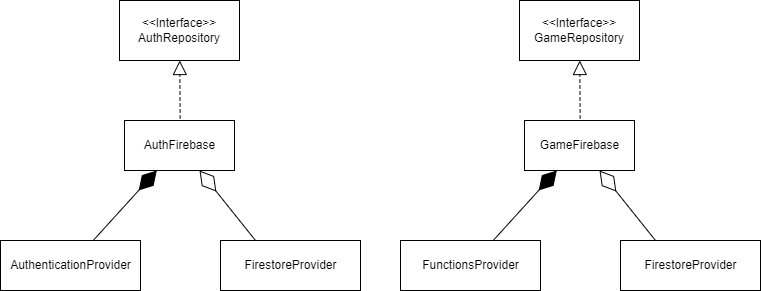
\includegraphics[width=16cm,height=6cm]{img/firebase-client.png}
	\end{center}
	\caption{{\color{dgray}Diagram klas warstwy danych firebase.}} 
	\label{firebase}
\end{figure}  
Klasa \emph{AuthFirebase} jest w relacji z klasą \emph{AuthenticationProvider} w postaci agregacji całkowitej (kompozycji). Oznacza to, że klasa główna (\emph{AuthFirebase}) ma na własność klasę częściową (\emph{AuthenticationProvider}) i kontroluje cykl życia części. Natomiast pomiędzy \emph{AuthFirebase}, a \emph{FirestoreProvider} występuje relacja agregacji częściowej. To znaczy, że element częściowy (\emph{FirestoreProvider}) należy do elementu głównego (\emph{AuthFirebase}), ale nie jest od niego zależny. Usunięcie elementu głównego, nie wpłynie na element częściowy. W przypadku \emph{GameFirebase} występuje ona w relacji częściowej z \emph{FirestoreProvider}, a w relacji agregacji całkowitej z \emph{FirestoreProvider}. Zatem z klasy \emph{FirestoreProvider} korzysta się w obu klasach implementujących interfejsy warstwy danych. \\ 
Klasa \emph{AuthenticationProvider} odpowiada za połączenie się z usługą \emph{Firebase Authentication} i przeprowadzanie operacji zarejestrowania, zalogowania i wylogowania użytkownika. \\
Klasa \emph{FirestoreProvider} odpowiada za połączenie się z usługą \emph{Firebase Firestore} (baza danych czasu rzeczywistnego). Klasa ta czyta lub zapisuje dane do bazy danych. Ponadto tworzy strumienie, które nasłuchują zmiany zachodzące w wybranych miejscach w bazie danych. \\
Klasa \emph{FunctionsProvider} odpowiada za połączenie się z usługą \emph{Firebase Functions}. Wywołuje dedykowane funkcje po stronie serwera. \\
W przypadku bota zdefiniowana jest jedna klasa \emph{GameBot}, która implementuje interfejs \emph{GameRepository}. Klasa ta zarządza instancją gry, która jest tworzona lokalnie na urządzeniu użytkownika. Biorąc pod uwagę rozwiązanie w postaci bota, konto użytkownika nie jest w użyciu. 
\begin{figure}[h!]
	\begin{center}
		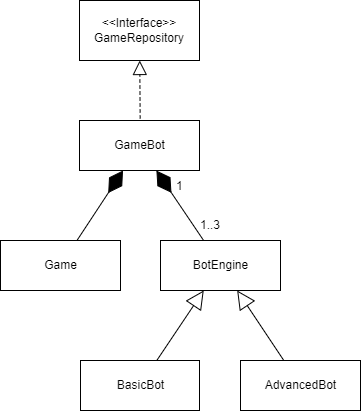
\includegraphics[width=8cm,height=9cm]{img/bot-client.png}
	\end{center}
	\caption{{\color{dgray}Diagram klas warstwy danych bot.}} 
	\label{bot}
\end{figure}

Klasa \emph{GameBot} występuje w relacji agregacji całkowitej z klasami \emph{Game} oraz \emph{BotEngine}. Klasa główna może zawierać od 1 do 3 instancji klasy \emph{BotEngine}. To ograniczenie wzięło się z zasady, że w grę Rummikub może grać od 2 do 4 graczy. Klasy \emph{BasicBot} i \emph{AdvancedBot} dziedziczą po klasie \emph{BotEngine}. \\
Klasa \emph{Game} jest instancją gry. Tworzy wszystkie możliwe kości w grze i losowo przydziela każdemu uczestnikowi. Przechowuje w sobie listę dostępnych kości do rozdania, listę kości przypisanych każdemu graczowi oraz zbiór zestawów kości, które są obecnie na planszy. \\
Klasa \emph{BotEngine} ma na celu imitować prawdziwego gracza. Analizuje obecny układ kości na plaszy oraz swoje własne kości i na tej podstawie wykonuje wyłożenie. Klasy \emph{BasicBot} oraz \emph{AdvancedBot} różnią się zaimplementowanym algorytmem wykonującym ruch. Algorytmy te wraz z opisem złożoności gry są przedstawione w następnym rozdziale.

\subsection{Przepływ zdarzeń}

W poprzednich podrozdziałach przedstawiono opisy poszczególnych warstw. W ostatnim podrozdziale zostały ukazane przepływy zdarzeń pomiędzy warstwami, aby zobrazować mechanikę działania systemu. Do przedstawienia graficznego wykorzystano diagramy sekwencji w notacji UML.

\begin{figure}[h!]
	\begin{center}
		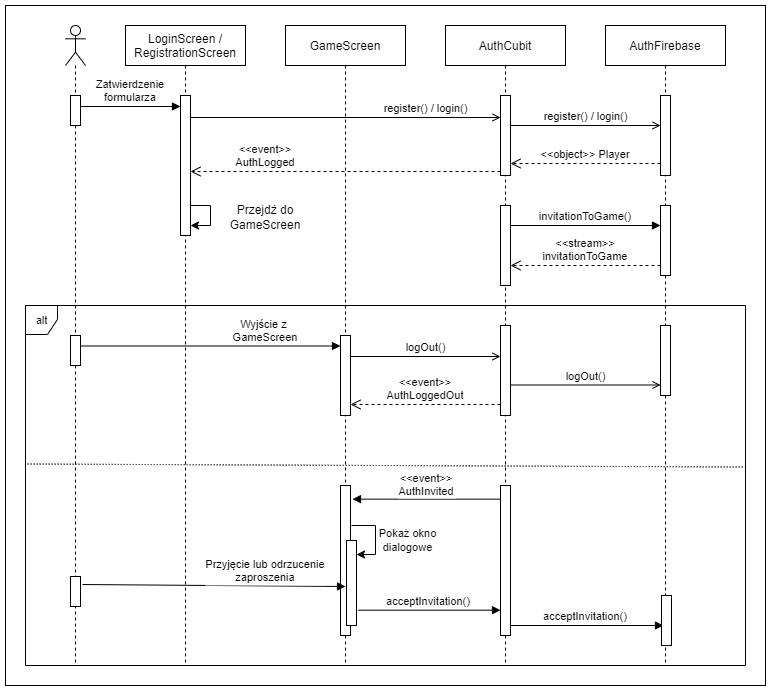
\includegraphics[width=16cm,height=12cm]{img/diagram-sekwencji-auth.png}
	\end{center}
	\caption{{\color{dgray}Diagram sekwencji AuthCubit.}} 
	\label{AuthCubit}
\end{figure}  


	\cleardoublepage
	
	\chapter{Bot}
\thispagestyle{chapterBeginStyle}

W ostatnim rozdziale przedstawiono analizę złożoności gry Rummikub oraz jakie podejścia zostały zrealizowane do implementacji bota . Podczas rozważania złożoności gry oraz implementacji skorzystano z artykułu ,,The Complexity of Rummikub Problems'' \cite{RummikubComplexity}. W związku z zastosowaniem architektury trójwarstwowej po stronie klienta bot zastępuje  warstwę danych bez konieczności modyfikowania logiki aplikacji.

\section{Podstawowy bot}

Implementacja podstawowego bota miała na celu umożliwienie przeprowadzanie rozgrywek na niskim poziomie trudności. Jest on przeznaczony dla osób, które dopiero poznają grę Rummikub. Jego zasada działania polega na formowaniu serii oraz grup z własnego zbioru kości. Bot ponadto potrafi modyfikować zbiory znajdujące się na planszy poprzez dodanie swoich kości na początek lub na koniec danego zbioru.

\section{Złożoność gry}

Gra Rummikub składa się z 106 kości, w których są dwa jokery. Joker może reprezentować sobą dowolną inną kość. Zatem 104 kości są numerowane od 1 do 13, w czterech różnych kolorach i każda kość występuje dwa razy. Kości można grupować w sekcje (rosnący ciąg liczb o tym samym kolorze) lub w grupy (kości o takiej samej liczbie z różnymi kolorami). Problemem jest znalezienie najlepszego wyłożenia podczas danego ruchu. \\

 Liczbę sposobów ułożenia grup z danej puli kości oznaczono jako $G(k, m)$, gdzie $k$ to jest liczba kolorów, a $m$ to jest liczba kopii. Na początek wzięto pod rozważanie przypadek, gdy $k = 4$, a $m = 1$. W takim przypadku dla danej wartości kości można nie formować żadnej grupy, formować cztery grupy o długości trzy lub jedną o długości cztery. Zatem $G(4,1) = 1 + {{4}\choose{3}} + 1 = 6$. W przypadku, gdy $m = 2$ pojawia się kopia każdej kości, a zatem są dwa zestawy, dla których można policzyć $G(4,1)$. Czyli $G(4,2) < G(4,1)^2$. Jest to górna granica, ponieważ pewne przypadki zostaną policzone więcej niż raz. Podczas tworzenia grup nie bierze się pod uwagę kolejności w jakiej te grupy są tworzone oraz przypadki, które łącznie dają taki sam zbiór kości, nie powinny być rozróżnialne. Pomimo tego liczba możliwych sposobów utworzenia grup rośnie nadal wykładniczo powołując się na artykuł \cite{RummikubComplexity}. Z tego powodu w implementacji algorytmu na początku formuje się serie, a dopiero później grupy z pozostałych kości. \\

Wybierając podejście, w którym najpierw formułuje się serie, a później grupy, dzieli się zbiór wszystkich kości (plansza oraz kości gracza) ze względu na wartość danej kości. Dla każdego podzbioru w kolejności od kości o wartościach $1$ aż do wartości $13$ tworzy się wszystkie możliwe kombinacje użycia poszczególnych kości do danych serii. Natomiast z kości, które pozostały w podzbiorach tworzy się możliwie jak największe grupy. \\

Zatem wystarczy dla każdego podzbioru o danej wartości kości, zdefiniować wszystkie możliwe do uzyskania konfiguracje serii. Aby seria spełniała zasady gry musi mieć co najmniej długość $3$. Z tego powodu poszczególne serie koduje się za pomocą cyfr $0$, $1$, $2$, $3$.  Wszystkie serie o długości powyżej $3$ koduje się jako $(3)$ w celu optymalizacji liczebności serii. Poszczególny stan gry będzie przedstawiony w postaci \emph{[wartość, konfiguracje serii]}. \\

W grze Rummikub jest możliwe stworzenie ośmiu pełnych serii (zbiór kości 1-13). Z tego powodu, że występują cztery kolory oraz każda kość ma swoją kopię. Zatem stan gry będzie określony jako $[v, abcdefgh]$, gdzie $v \in \{1..13\}$, a $(a, b, c, d, e, f, g, h) \in \{0, 1, 2, 3\}$. Założono, że $(a, b)$ przedstawiają serie koloru czarnego, $(c, d)$ koloru niebieskiego, $(e, f)$ koloru pomarańczowego, $(g, h)$ koloru czerwonego. Serie kości $(2, 3, 4, 5)$ koloru niebieskiego oraz $(1, 2, 3)$ koloru czerwonego będą zakodowane w następujący sposób: $$[1, 00000001], [2, 00010002], [3, 00020003], [4, 00030000], [5, 00030000], [6, 00000000]$$

\section{Zaawansowany bot}

Podczas implementacji bota zmodyfikowano algorytm opisany w artykule \cite{RummikubComplexity}. $MaxScore$ oprócz zwracania największej możliwej sumy wszystkich wartości kości, zwraca również wybraną konfiguracje serii oraz gwarantuje, że wszystkie kości na planszy będą ponownie wykorzystane. \\

\begin{pseudokod}[H]
	\SetAlTitleFnt{small}
	\SetArgSty{normalfont}
	\SetKwFunction{MakeRuns}{MakeRuns}
	\SetKwFunction{GetRunScores}{GetRunScores}
	\SetKwFunction{GetGroupScores}{GetGroupScores}
	\SetKwFunction{MaxScore}{MaxScore}
	\KwIn{$value, runs, tableTiles$}
	\KwOut{$result[value, runs]$}
	\vskip 1mm
	\If{$value > 13$}{
		\textbf{return} $null$;
	}
	\If{$result[value, runs] \neq null$}{
		\textbf{return} $result[value, runs]$;
	}
	$scores \leftarrow -\infty$\;
	\For{$possibleRuns \in \MakeRuns{value, runs}$}{
		$runScores \leftarrow \GetRunScores{possibleRuns, runs, tableTiles, tiles, value}$\;
		$groupScores \leftarrow \GetGroupScores{tiles, value}$\;
		\If{$runScores = -1$ or $groupScores = -1$}{
			\textbf{continue};
		}
		$maxScore \leftarrow \MaxScore{value + 1, possibleRuns, tableTiles}$\;
		$sum \leftarrow runScores + groupScores + maxScore[scores]$\;
		\If{$scores < sum$}{
			$scores \leftarrow sum$\;
			$result[value, runs] \leftarrow [sum, possibleRuns]$\;	
		}
	}
	\caption{MaxScore}\label{alg:mine}
\end{pseudokod}
\vskip 3mm

Na początku algorytmu sprawdzane jest czy dana wartość $value$ nie przekroczyła maksymalnej wartości kości oraz czy dany stan gry nie został już poprzednio obliczony. Następnie następuje iteracja po wszystkich możliwych nowych konfiguracjach serii. Funkcja $MakeRuns$ tworzy nowe konfiguracje na podstawie obecnej konfiguracji serii i dostępnych kościach o wartości $value$. Funkcja $GetRunScores$ oblicza punkty na podstawie porównania nowej konfiguracji $possibleRuns$ z poprzednią $runs$. Ponadto usuwa ze zbioru $tiles$, użyte kości do utworzenia nowej konfiguracji serii. W przypadku gdyby seria o długości mniejszej niż trzy zawierające kości należące do planszy zostałaby przerwana, $GetRunScores$ zwróci wartość $-1$. $GetGroupScores$ z kolei tworzy grupy o największej liczbie punktów, usuwa użyte kości ze zbioru $tiles$ i w przypadku gdy pozostaną kości należące do planszy również zwraca $-1$. Następnie jest wywoływana rekurencyjnie funkcja $MaxScore$, której przekazywana wartość kości powiększona o jeden, nowa konfiguracja kości oraz zmodyfikowana tablica $tableTiles$. Po zsumowaniu wyniku sprawdzane jest, czy otrzymywany wynik jest obecnie największym możliwym wynikiem dla tego stanu gry.
Najlepszy wynik otrzymany w poszczególnym stanie jest zapisywany do tablicy wszystkich stanów wraz z konfiguracją serii, która została wybrana dla tego stanu. \\

Po wykonanej rekurencji algorytm zwraca najlepszy możliwy wynik oraz pierwszą wybraną konfigurację serii. Dzięki temu, że dla każdej wartości $value$ wynik jest zapisywany do tablicy $result$ z indeksem $[value, runs]$ można odtworzyć przebieg konfiguracji serii. Zatem iterując po wszystkich wartościach $value$ można odtworzyć utworzone serie oraz grupy.




	\cleardoublepage
	
	\chapter*{Podsumowanie}
\addcontentsline{toc}{chapter}{Podsumowanie}
\thispagestyle{chapterBeginStyle}

Obecnie serwis jest gotowy do wdrożenia. Wszystkie wskazane funkcjonalności zostały zaimplementowane. Serwis działa zarówno na stronie w przeglądarce jak i w postaci aplikacji mobilnej na telefon z systemem Android. Użytkownicy mogą zakładać własne konta i grać z innymi użytkownikami przez internet lub z botem bez potrzeby zakładania konta i łączności z internetem. \\

Główny fundament serwisu został stworzony, więc teraz można rozszerzać serwis o nowe funkcjonalności. Najbardziej pożądaną kwestią jest dodanie bota po stronie serwera. Funkcjonalność ta przydałaby się w momencie, gdy chcemy zagrać w grę z większą liczbą osób, a niestety w pewnej chwili w serwisie nie ma zbyt wielu graczy. Ponadto należałoby rozwinąć możliwości związane z kontami użytkowników. Udostępniać statystyki dotyczące danego użytkownika, wprowadzić możliwość komunikacji tekstowej między graczami. Warto byłoby też pochylić się nad ulepszeniem wizualizacji aplikacji (dodaniem animacji czy efektów głosowych). \\

W projekcie tym udało się pomyślnie wykorzystać technologie Flutter oraz Firebase. Wymagało to przeznaczenia pewnej ilości czasu na ich naukę z uwagi na to, że są to dosyć młode technologie oraz serwis ten jest pierwszym większym projektem korzystającym z tych technologii dla autora. Z pewnością zapoznanie się z wieloplatformową technologią budowania aplikacji było cennym doświadczeniem. Wartością dodaną tego projektu jest szczególnie możliwość zapoznania się ze złożonością gry Rummikub.
	\cleardoublepage
	
	
	%%%%%%%%%%%%%%%%%%%%%%%%%%%%%%%%%%%%%%%%%%%%%%%%%%%%%%%%%%%%%%%%%%%%%%%%%%%%%%
	%%%%%%%%%%%%%%%%%%%%%%%%%%%%%%% BIBLIOGRAFIA %%%%%%%%%%%%%%%%%%%%%%%%%%%%%%%%%
	%%%%%%%%%%%%%%%%%%%%%%%%%%%%%%%%%%%%%%%%%%%%%%%%%%%%%%%%%%%%%%%%%%%%%%%%%%%%%%

	\pagestyle{bibliographyStyle}
	\bibliographystyle{plabbrv}
	\bibliography{literatura}
	\thispagestyle{chapterBeginStyle}
        \addcontentsline{toc}{chapter}{Bibliografia}
	\cleardoublepage
	
	%%%%%%%%%%%%%%%%%%%%%%%%%%%%%%%%%%%%%%%%%%%%%%%%%%%%%%%%%%%%%%%%%%%%%%%%%%%%%%
	%%%%%%%%%%%%%%%%%%%%%%%%%%%%%%%%% DODATKI %%%%%%%%%%%%%%%%%%%%%%%%%%%%%%%%%%%%
	%%%%%%%%%%%%%%%%%%%%%%%%%%%%%%%%%%%%%%%%%%%%%%%%%%%%%%%%%%%%%%%%%%%%%%%%%%%%%%
	
	\appendix
	\pagestyle{appendixStyle}
       \renewcommand{\appendixname}{Załącznik}
	
	\chapter{Zawartość płyty CD}
\thispagestyle{chapterBeginStyle}
\label{plytaCD}

Do pracy dyplomowej została dołączana płyta CD, na której znajduje się projekt zawierający kod źródłowy zaimplementowanego serwisu. Zamieszczony został również plik binarny (o rozszerzeniu apk) umożliwiający instalację aplikacji na telefonie z systemem Android. Ponadto umieszczone zostały zdjęcia obrazujące wygląd serwisu.


	
	\cleardoublepage

\end{document}

